\section{Results}
\label{sec:results}

\subsection{All Styles Are Linearly Represented}

\Tabref{tab:probing} shows probing results at each style's best layer. Non-linearity indices range from 0.965 (sadness) to 1.008 (curiosity), with a mean of 0.991. The MLP probe does not outperform the linear probe for any style at any layer. This result is unambiguous: \pythia represents all 11 tested emotions as linear directions in activation space.

\begin{table}[t]
    \centering
    \caption{Probing results at the best layer per style. Linear and MLP probe accuracies are reported with the non-linearity index (NL Index $=$ MLP/Linear). NL Index $\approx 1.0$ for all styles indicates uniformly linear representations. Best linear probe accuracy in \textbf{bold}.}
    \label{tab:probing}
    \begin{tabular}{@{}lcccc@{}}
        \toprule
        Style & Layer & Linear Acc. & MLP Acc. & NL Index \\
        \midrule
        \textbf{Gratitude} & 16 & \textbf{0.970} & 0.954 & 0.984 \\
        Love & 4 & 0.939 & 0.934 & 0.995 \\
        Fear & 4 & 0.900 & 0.881 & 0.980 \\
        Surprise & 8 & 0.892 & 0.895 & 1.003 \\
        Joy & 4 & 0.872 & 0.855 & 0.981 \\
        Admiration & 8 & 0.872 & 0.874 & 1.002 \\
        Sadness & 4 & 0.856 & 0.826 & 0.965 \\
        Disgust & 4 & 0.847 & 0.827 & 0.976 \\
        Curiosity & 20 & 0.831 & 0.838 & 1.008 \\
        Anger & 12 & 0.826 & 0.828 & 1.002 \\
        Confusion & 12 & 0.807 & 0.809 & 1.002 \\
        \bottomrule
    \end{tabular}
\end{table}

Despite uniform linearity, linear separability varies substantially across styles. Gratitude (0.970) and love (0.939) are the most separable, while confusion (0.807) and anger (0.826) are the least. This 0.16-point range reflects genuine differences in how distinctly each style is encoded.

\para{Layer-wise patterns.} Most styles achieve peak probe accuracy at early layers (layer~4), but gratitude peaks at layer~16 and curiosity at layer~20, suggesting that some emotional dimensions are computed in deeper layers. \Figref{fig:probes} shows the comparison of linear and MLP probes across styles.

\begin{figure}[t]
    \centering
    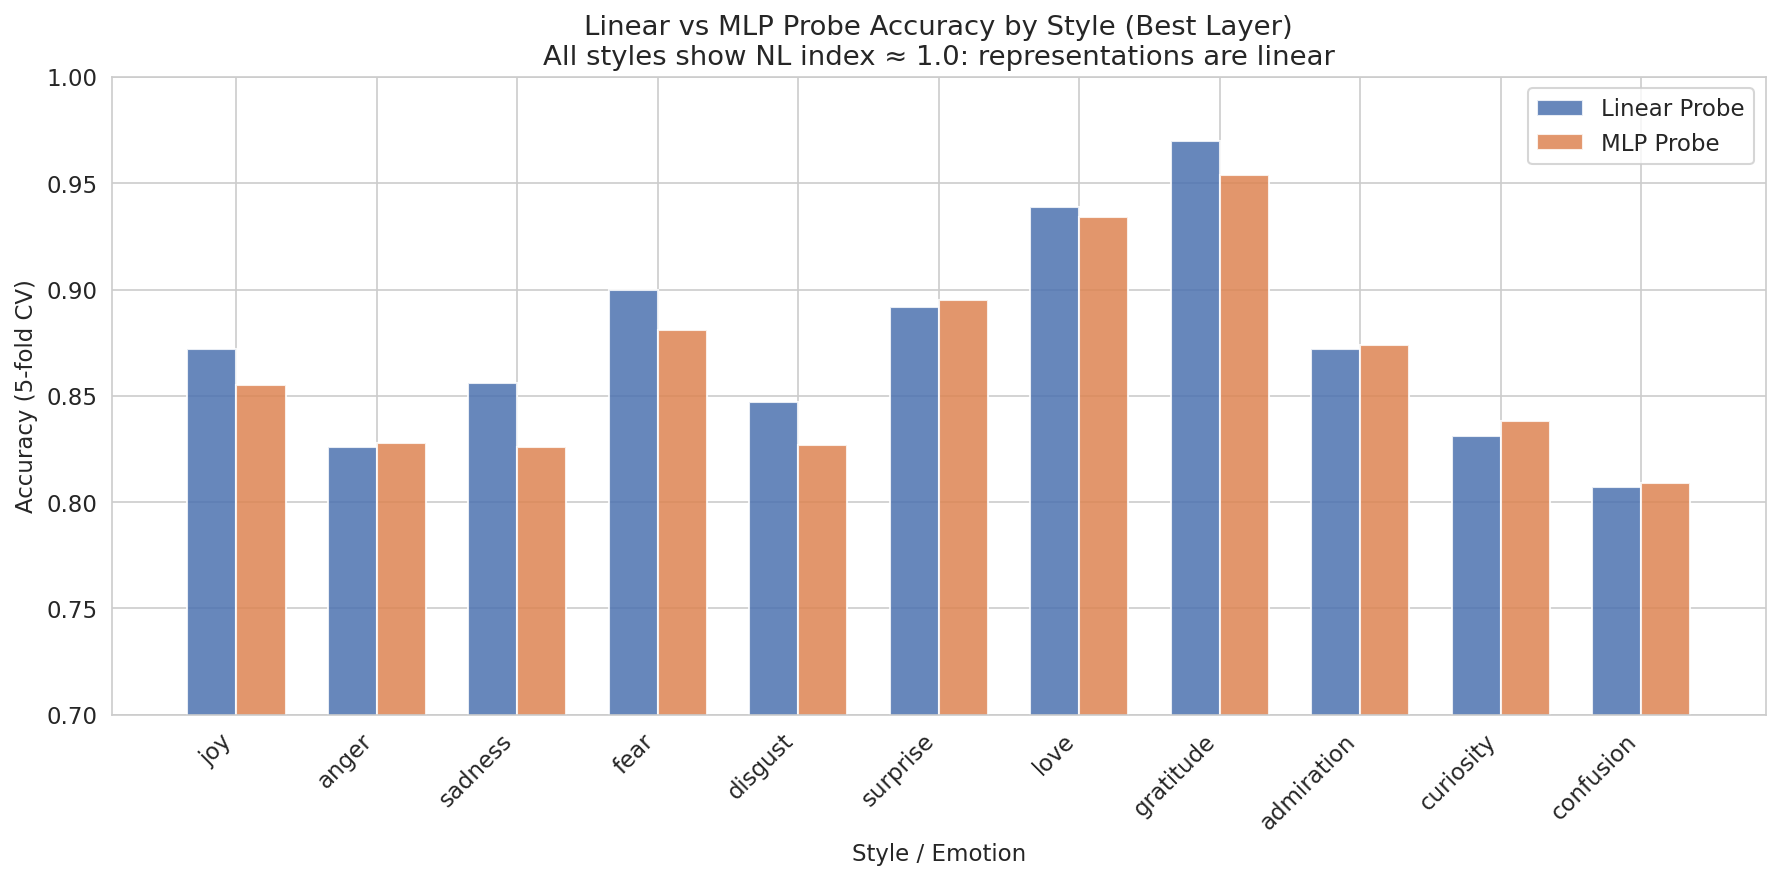
\includegraphics[width=0.95\linewidth]{figures/01_linear_vs_mlp_probes.png}
    \caption{Linear versus MLP probe accuracy for each style. The two probe types achieve nearly identical accuracy across all styles, with non-linearity indices clustered tightly around 1.0. This indicates that MLP probes extract no additional information beyond what linear probes capture.}
    \label{fig:probes}
\end{figure}

\subsection{Steering Effectiveness Is Independent of Linear Separability}

\Tabref{tab:steering} presents steering results. Cohen's $d$ ranges from 0.090 (fear) to 0.907 (sadness), and generation shift ranges from $-0.067$ to $+0.733$. The correlation between linear probe accuracy and Cohen's $d$ is $r = -0.220$ ($p = 0.52$)---weak and non-significant.

\begin{table}[t]
    \centering
    \caption{Steering results for each style. Cohen's $d$ measures activation-space separation; generation shift measures the change in style classification rate relative to unsteered baseline. Largest generation shifts in \textbf{bold}. Linear separability does not predict either metric.}
    \label{tab:steering}
    \begin{tabular}{@{}lccccc@{}}
        \toprule
        Style & Cohen's $d$ & SV Acc. & Baseline & Steered & Shift \\
        \midrule
        Gratitude & 0.381 & 0.569 & 0.067 & 0.800 & \textbf{+0.733} \\
        Fear & 0.090 & 0.499 & 0.400 & 0.800 & +0.400 \\
        Love & 0.147 & 0.512 & 0.200 & 0.533 & +0.333 \\
        Joy & 0.634 & 0.620 & 0.333 & 0.600 & +0.267 \\
        Anger & 0.129 & 0.504 & 0.133 & 0.400 & +0.267 \\
        Confusion & 0.455 & 0.587 & 0.333 & 0.600 & +0.267 \\
        Disgust & 0.129 & 0.510 & 0.400 & 0.533 & +0.133 \\
        Curiosity & 0.525 & 0.604 & 0.200 & 0.333 & +0.133 \\
        Sadness & 0.907 & 0.673 & 0.333 & 0.267 & $-$0.067 \\
        Surprise & 0.163 & 0.539 & 0.467 & 0.400 & $-$0.067 \\
        Admiration & 0.192 & 0.534 & 0.600 & 0.533 & $-$0.067 \\
        \bottomrule
    \end{tabular}
\end{table}

Several results are noteworthy. Sadness has the highest Cohen's $d$ (0.907) yet a \emph{negative} generation shift ($-0.067$): the mean-difference vector points in a direction that is linearly separable but not causally effective for generation. Fear has the lowest Cohen's $d$ (0.090) yet the second-largest generation shift (+0.400), suggesting that even weak steering vectors can cause large behavioral shifts when they align with sensitive decision boundaries. Gratitude achieves the largest generation shift (+0.733) despite only moderate activation-space separation ($d = 0.381$).

\para{Random vector control.} Random vectors of the same norm produce negligible style projection changes ($-0.023$ for joy, $-0.241$ for anger, $-0.028$ for sadness), confirming that real steering vectors carry style-specific information (\figref{fig:steering}).

\begin{figure}[t]
    \centering
    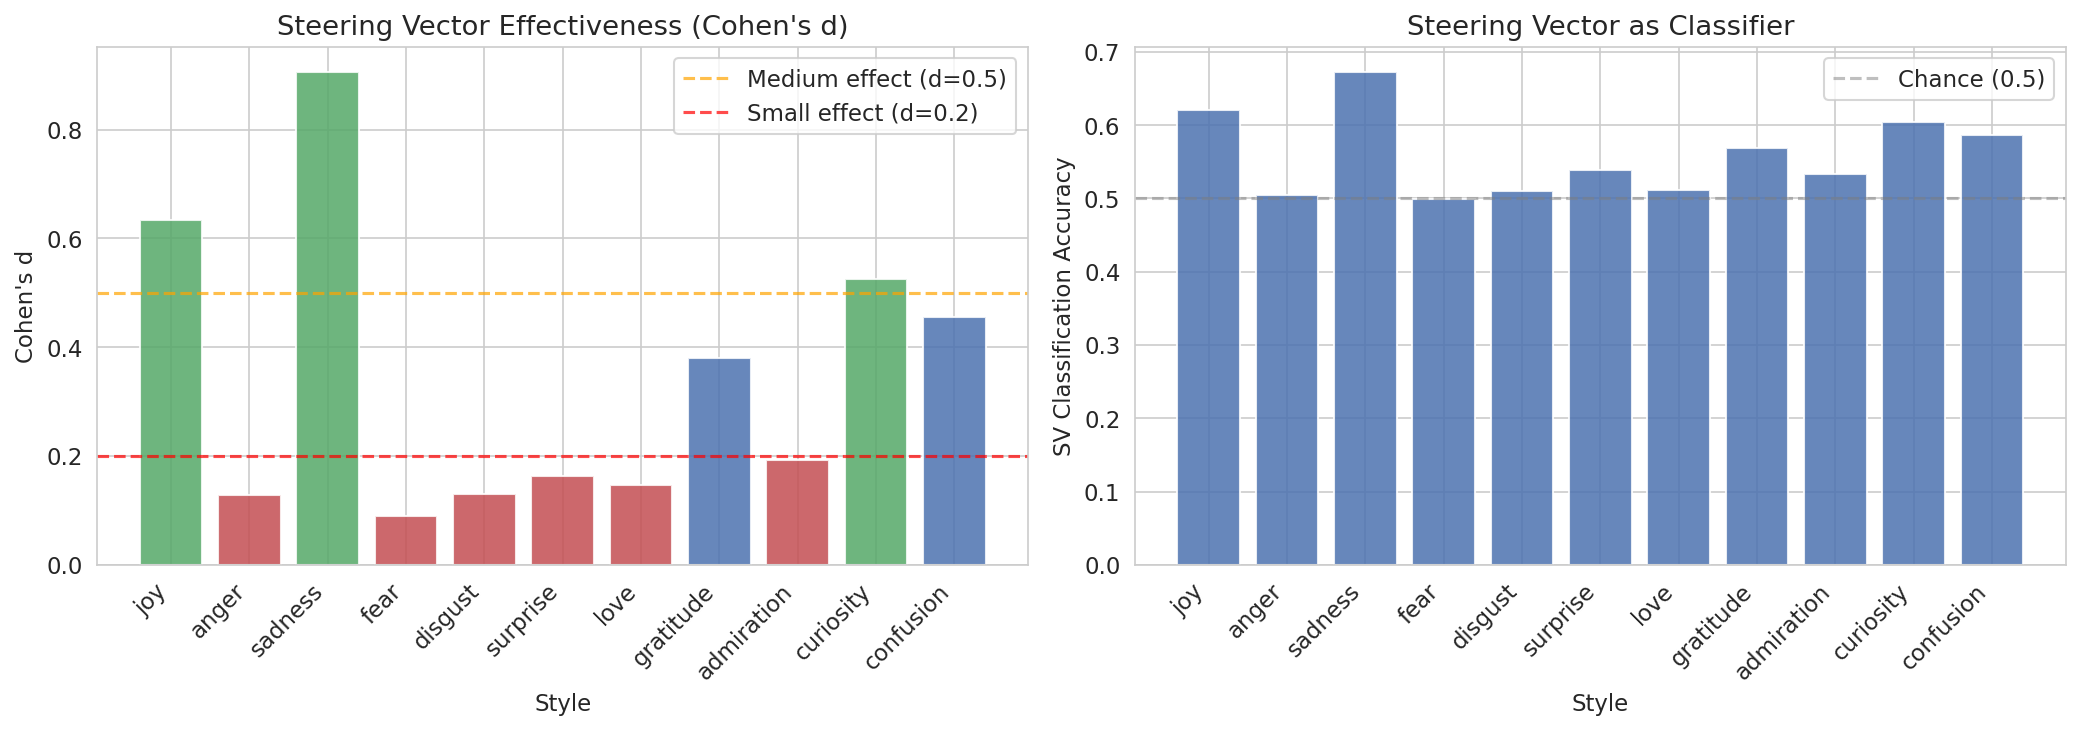
\includegraphics[width=0.95\linewidth]{figures/06_steering_effectiveness.png}
    \caption{Steering effectiveness measured by Cohen's $d$ and steering vector classification accuracy per style. Styles with high activation-space metrics (sadness) do not necessarily produce positive generation shifts, while styles with low metrics (fear) sometimes do.}
    \label{fig:steering}
\end{figure}

\subsection{Prompting Succeeds Uniformly}

\Tabref{tab:prompting} shows prompting results. All 11 styles achieve 100\% success rate ($\geq 3/5$ adherence score) with mean adherence ranging from 3.8 (confusion) to 4.4 (joy, disgust, gratitude). Specificity scores confirm that prompted text is rated higher for the target style than for a random alternative style.

\begin{table}[t]
    \centering
    \caption{Prompting results using GPT-4.1-nano. Target score is the mean style adherence rating (1--5). Specificity is the difference between target style rating and random alternative style rating. All styles achieve 100\% success rate. Best target scores in \textbf{bold}.}
    \label{tab:prompting}
    \begin{tabular}{@{}lccc@{}}
        \toprule
        Style & Target Score & Success Rate & Specificity \\
        \midrule
        Joy & \textbf{4.40} & 100\% & +3.30 \\
        Disgust & \textbf{4.40} & 100\% & +0.70 \\
        Gratitude & \textbf{4.40} & 100\% & +2.20 \\
        Surprise & 4.10 & 100\% & +1.90 \\
        Anger & 4.00 & 100\% & +2.40 \\
        Sadness & 4.00 & 100\% & +1.80 \\
        Fear & 4.00 & 100\% & +1.50 \\
        Love & 4.00 & 100\% & +3.00 \\
        Admiration & 4.00 & 100\% & +3.00 \\
        Curiosity & 3.90 & 100\% & +0.70 \\
        Confusion & 3.80 & 100\% & +1.80 \\
        \bottomrule
    \end{tabular}
\end{table}

Notably, disgust---historically the hardest style to steer \citep{konen2024style}---achieves the joint-highest prompting score (4.4/5). This directly demonstrates that steering difficulty does not predict prompting difficulty.

\subsection{The Three Measures Are Independent}

\Tabref{tab:correlations} presents the full correlation matrix across our three measurement dimensions. No correlation reaches statistical significance.

\begin{table}[t]
    \centering
    \caption{Pearson correlations between probing, steering, and prompting metrics. None reach statistical significance ($\alpha = 0.05$), indicating that the three measures capture largely independent dimensions of style encoding.}
    \label{tab:correlations}
    \begin{tabular}{@{}lcc@{}}
        \toprule
        Correlation & Pearson $r$ & $p$-value \\
        \midrule
        Linear acc. $\leftrightarrow$ Prompt score & 0.447 & 0.168 \\
        Linear acc. $\leftrightarrow$ Prompt specificity & 0.359 & 0.278 \\
        NL index $\leftrightarrow$ Prompt score & $-$0.515 & 0.105 \\
        Cohen's $d$ $\leftrightarrow$ Linear acc. & $-$0.220 & 0.516 \\
        Cohen's $d$ $\leftrightarrow$ Prompt score & $-$0.018 & 0.957 \\
        SV acc. $\leftrightarrow$ Prompt score & $-$0.029 & 0.932 \\
        \bottomrule
    \end{tabular}
\end{table}

The most striking result is the near-zero correlation between steering effectiveness and prompting success ($r = -0.018$, $p = 0.96$). \Figref{fig:scatter} visualizes this relationship. The three measures---linear separability, steerability, and promptability---are largely independent dimensions of how the model encodes and accesses style information.

\begin{figure}[t]
    \centering
    \begin{subfigure}[b]{0.48\textwidth}
        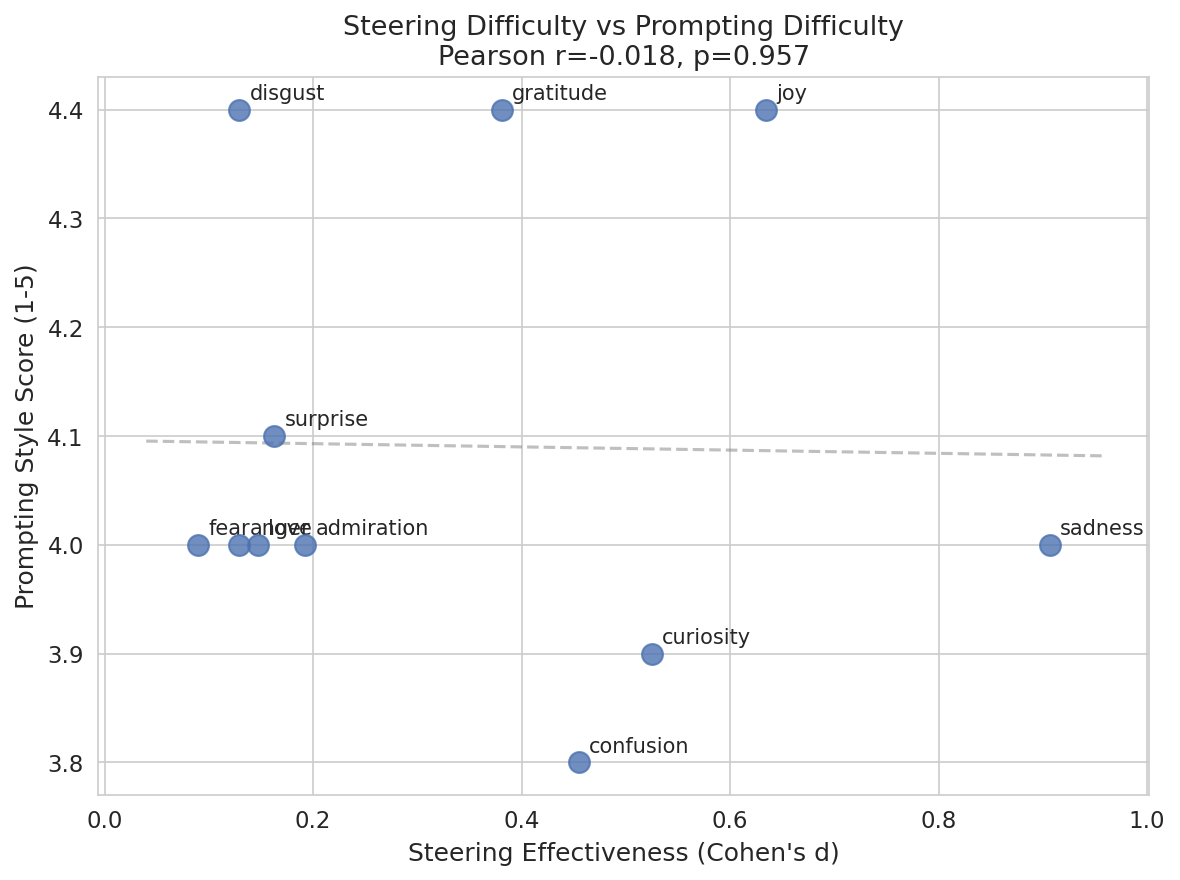
\includegraphics[width=\textwidth]{figures/07_steering_vs_prompting.png}
        \caption{Steering vs.\ prompting}
        \label{fig:steer_vs_prompt}
    \end{subfigure}
    \hfill
    \begin{subfigure}[b]{0.48\textwidth}
        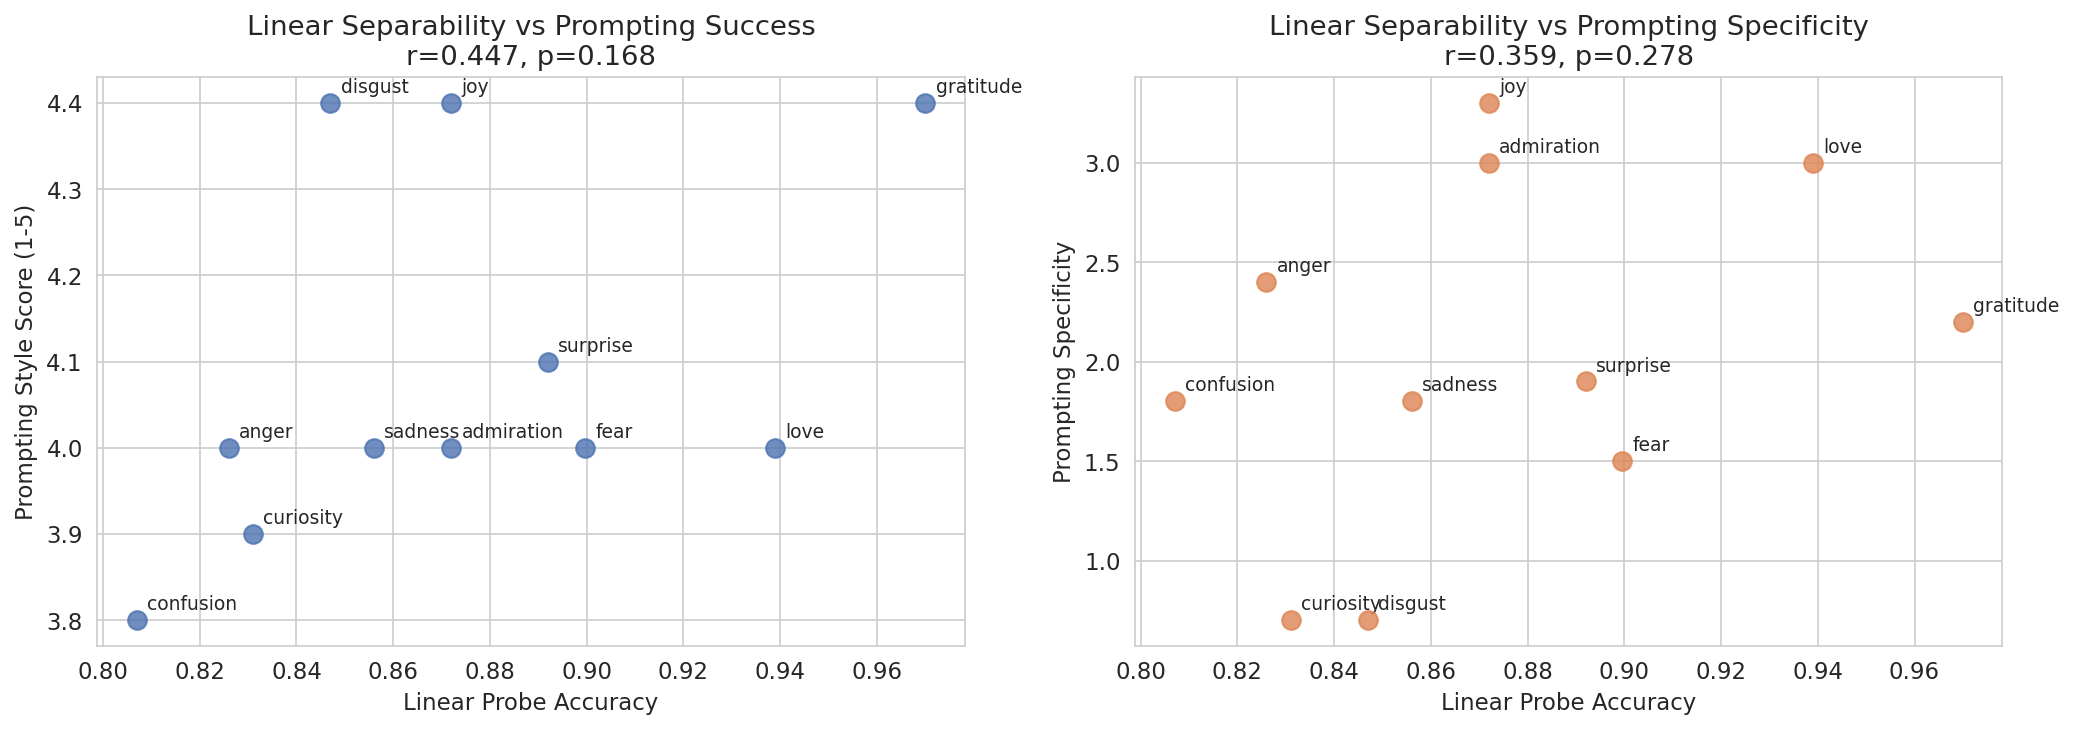
\includegraphics[width=\textwidth]{figures/05_linearity_vs_prompting.png}
        \caption{Linearity vs.\ prompting}
        \label{fig:lin_vs_prompt}
    \end{subfigure}
    \caption{\figleft Steering effectiveness (Cohen's $d$) versus prompting adherence score for each style. The near-zero correlation ($r = -0.018$) shows these access fundamentally different pathways. \figright Linear probe accuracy versus prompting score; the weak positive trend ($r = 0.447$) is not significant.}
    \label{fig:scatter}
\end{figure}
